\documentclass[margin=0.5cm]{standalone}
\usepackage{tikz}
\usetikzlibrary{positioning,shadows,shapes,arrows}
\begin{document}
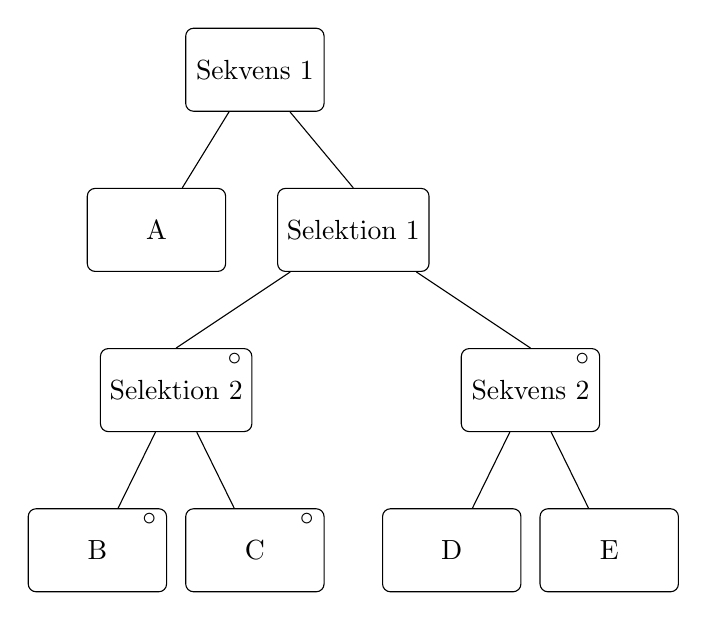
\begin{tikzpicture}[
    box/.style={
        rectangle,
        draw=black,
        rounded corners=1mm,
        minimum width=5em,
        minimum height=3em,
        level distance=10cm,
        text centered,
        anchor=north,
        align=center
    },
    circle/.style={
        rectangle,
        draw=black,
        rounded corners=1mm,
        minimum width=5em,
        minimum height=3em,
        level distance=10cm,
        text centered,
        anchor=north,
        label={[xshift=-1.25em, yshift=-2.25ex]north east:$\circ$},
        align=center
    },
]
    \node (JSP) [box] {Sekvens 1}
     [sibling distance=2.5cm]
        child {node (a) [box] {A}}
        child {[sibling distance=4.5cm] node (b) [box] {Selektion 1}
          child {[sibling distance=2cm] node (c) [circle] {Selektion 2}
            child {node (d) [circle] {B}}
            child {node (e) [circle] {C}}
          }
          child {[sibling distance=2cm] node (f) [circle] {Sekvens 2}
            child {node (g) [box] {D}}
            child {node (h) [box] {E}}
          }
        }
    ;
\end{tikzpicture}
\end{document}
